\documentclass[11pt,letterpaper]{article}

\usepackage[margin=1in]{geometry}
\usepackage{enumitem}
\usepackage{hyperref}
\usepackage{amsmath}
\usepackage{tikz}
\usetikzlibrary{decorations.pathmorphing, decorations.pathreplacing, calc}

\title{16.07 Dynamics Problem Set 1}
\author{Due Friday, September 25}
\date{}

\begin{document}

\maketitle

\section{Spring-Loaded Inverted Pendulum Dynamics}

\begin{figure}[h]
\centering
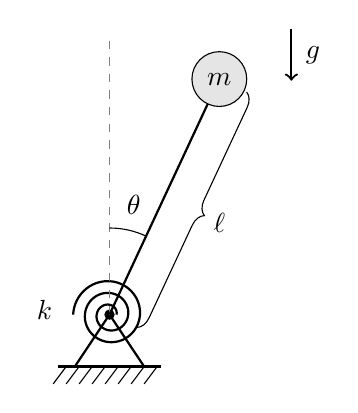
\begin{tikzpicture}[scale=1.1]
    \def\Lrod{3}
    \def\thetadeg{25}

    % --- Ground (fixed anchor) ---
    \draw[thick] (-0.6,-0.6) -- (0.6,-0.6);
    \foreach \x in {-0.5,-0.35,-0.2,-0.05,0.1,0.25,0.4,0.55}
        \draw (\x,-0.6) -- (\x-0.15,-0.8);

    % --- Support triangle (pin fixed to ground), apex at the pivot ---
    \draw[thick] (0,0) -- (-0.4,-0.6) -- (0.4,-0.6) -- cycle;

    % --- Torsion spring: flat spiral centered on the pivot ---
    \draw[thick] plot[domain=0:900, samples=150, variable=\t]
        ({(0.08+0.34*\t/900)*cos(\t)}, {(0.08+0.34*\t/900)*sin(\t)});
    \node at (-0.75,0.05) {$k$};

    % --- Pivot point ---
    \filldraw (0,0) circle (1.5pt);

    % --- Vertical reference (upright direction), dashed ---
    \draw[dashed, gray] (0,0) -- (0,3.2);

    % --- Rod at angle theta from vertical ---
    \coordinate (O) at (0,0);
    \coordinate (P) at ({\Lrod*sin(\thetadeg)},{\Lrod*cos(\thetadeg)});
    \draw[thick] (O) -- (P);

    % --- Mass at tip ---
    \filldraw[fill=gray!20] (P) circle (9pt);
    \node at (P) {$m$};

    % --- Angle arc, label centered on the arc ---
    \draw (0,1) arc (90:{90-\thetadeg}:1);
    \node at ({(1.3)*cos(90-\thetadeg/2)},{(1.3)*sin(90-\thetadeg/2)}) {$\theta$};

    % --- Length measurement: curly brace parallel to the rod, offset to its right ---
    \coordinate (Ob) at ({0.35*cos(\thetadeg)},{-0.35*sin(\thetadeg)});
    \coordinate (Pb) at ({\Lrod*sin(\thetadeg)+0.35*cos(\thetadeg)},{\Lrod*cos(\thetadeg)-0.35*sin(\thetadeg)});
    \draw[decorate, decoration={brace, amplitude=5pt, mirror}] (Ob) -- (Pb);
    \node at ($(Ob)!0.5!(Pb) + ({0.35*cos(\thetadeg)},{-0.35*sin(\thetadeg)})$) {$\ell$};

    % --- Gravity direction indicator ---
    \draw[->, thick] (2.1,3.3) -- (2.1,2.7);
    \node at (2.35,3.0) {$g$};
\end{tikzpicture}
\label{fig:pendulum}
\end{figure}

\noindent We'll be analyzing an inverted pendulum with a massless rod of length $\ell$, a point mass $m$ attached at the tip, and a torsion spring of stiffness $k$ mounted at the pivot. The spring is uncompressed when the rod is exactly vertical. Let $\theta$ be the angle measured from the upward vertical line, positive in the direction shown in the figure.

Derive the nonlinear equation of motion for this inverted pendulum using Newton's 2nd law as we did in class. Leave it in terms of the constants shown in the diagram for now --- we'll plug in numerical values later.

\section{Linearization and Stability}

Linearize the equation of motion from Section 1 for small $\theta$ using the small-angle approximation $\sin\theta \approx \theta$. Write the resulting linear, constant-coefficient, second-order ODE in the standard form:
\[
\ddot\theta + a \theta = 0
\]


\begin{enumerate}[label=(\alph*)]
    \item Assuming the linearized coefficient $a$ is positive, write the natural frequency $\omega_n$ of the system in terms of $m$, $g$, $\ell$, and $k$.
    \item Assume $m$, $\ell$, and $g$ are fixed but $k$ is a design parameter we can vary. Identify the values of $k$ for which the system is stable and unstable. Find the critical stiffness $k_{cr}$ where this stability transition occurs in terms of $m$, $g$, and $\ell$.
\end{enumerate}

\section{Energy Analysis}

\begin{enumerate}[label=(\alph*)]
    \item Write the kinetic energy $T(\theta,\dot\theta)$ and potential energy $U(\theta)$ of the system, including both the gravitational and torsional spring contributions.
    \item Assume $m=\ell=1$ and $g=9.8$. Using MATLAB or Python, plot $U(\theta)$ over the range $\theta \in [-3,3]$ rad for three values of $k$:
    \begin{itemize}
        \item $k = 0.5\,k_{cr}$
        \item $k = k_{cr}$
        \item $k = 1.5\,k_{cr}$
    \end{itemize}
    \item Equilibria are points where, if initialized at rest, the system will remain at rest (i.e. all forces sum to zero). What does this correspond to on your plots of $U(\theta)$? Identify and mark all equilibria on your three plots.
    \item Given what we already know about stability from our linear analysis, how can you determine stability from the potential $U(\theta)$? Indicate the stability of each equilibrium point graphically on your plots via color coding or using different marker styles.
    \item \textbf{Pay particular attention to the case $k = k_{cr}$.} Your natural-frequency expression from Section 3 gives $\omega_n = 0$ in this case --- by itself, this does \textbf{not} tell you whether $\theta = 0$ is stable or unstable. Using the shape of $U(\theta)$ near $\theta = 0$, what can you say about the true nonlinear stability of the upright equilibrium when $k = k_{cr}$? Explain in a sentence or two why the linearized analysis from Section 3 is insufficient to answer this question.
\end{enumerate}

\section{Numerical Simulation}

For each of the three values of $k$ from Section 4, numerically integrate the full nonlinear dynamics from Section 1 using \texttt{ode45} (MATLAB) or \texttt{scipy.integrate.solve\_ivp} (Python).

\begin{enumerate}[label=(\alph*)]
    \item For each $k$, run a batch of simulations (e.g., $\approx$20 runs) starting from the upright equilibrium with zero initial angular velocity ($\dot\theta(0) = 0$) and $\theta(0)$ drawn from a uniform distribution over a suitable range (e.g., $\theta(0) \sim U(-3,3)$ rad). Integrate each simulation long enough to see its long-term behavior clearly.
    \item For each value of $k$, plot all trajectories together on a single phase-plane plot ($\theta$ on the horizontal axis, $\dot\theta$ on the vertical axis). Verify and comment on your stability analysis for the case $k=k_{cr}$.
    \item A basin of attraction is the region of state space around a stable equilibrium point within which trajectories converge to the equilibrium. The dividing line between two basins is called a \emph{separatrix}. Identify and mark the separatrix on your phase plot for the $k = 0.5\,k_{cr}$ case. \emph{Hint:} The separatrix is actually a trajectory of the system, so you can identify appropriate initial conditions and simulate it to plot it. Verify that no trajectories cross this line.
\end{enumerate}

\end{document}
